\begin{circuitikz}
\tikzstyle{every node}=[font=\fontsize{14.2pt}{18.5pt}\selectfont]
\draw [ fill={rgb,255:red,243; green,243; blue,243}, fill opacity=1, rounded corners = 28.8, dashed] (5.375,17) rectangle (10.875,11);
\draw [ color={rgb,255:red,255; green,0; blue,0}, draw opacity=1, line width=1.5pt, -{Stealth[scale=1.5]}, ] (24.5,9.375) -- (16,9.375);
\draw [ color={rgb,255:red,255; green,0; blue,0}, draw opacity=1, line width=1.5pt, -{Stealth[scale=1.5]}, ] (17.625,13.75) -- (19.375,13.75);
\draw [line width=1.5pt, -{Stealth[scale=1.5]}, ] (12,17.375) -- (12,10.5);
\draw [ fill={rgb,255:red,255; green,255; blue,255}, fill opacity=1, line width=1pt , rounded corners = 20.4] (19.5,21.75) rectangle (30,12.75);
\draw [ fill={rgb,255:red,75; green,158; blue,207}, fill opacity=1, line width=1pt , rounded corners = 12.6] (19.5,21.75) rectangle (30,20.125);
\draw [ fill={rgb,255:red,255; green,255; blue,255}, fill opacity=1, line width=1pt , rounded corners = 20.4] (5.375,10.375) rectangle (15.875,1.375);
\draw [ fill={rgb,255:red,255; green,255; blue,255}, fill opacity=1, line width=1pt , rounded corners = 11.4] (18.875,8.125) rectangle (30,1.5);
\draw [-{Stealth[scale=1.5]}, short] (27.25,3.125) -- (27.25,6.5);
\draw [ fill={rgb,255:red,75; green,158; blue,207}, fill opacity=1, line width=1pt , rounded corners = 12.6] (18.875,8.25) rectangle (30,6.625);
\draw [short] (10.875,10.375) -- (10.875,8.125);
\draw [ fill={rgb,255:red,75; green,158; blue,207}, fill opacity=1, line width=1pt , rounded corners = 12.6] (5.375,10.375) rectangle (15.875,8.75);
\draw [ fill={rgb,255:red,255; green,255; blue,255}, fill opacity=1, rounded corners = 40.2] (9.375,21.125) rectangle (14.875,17.125);
\draw [ color={rgb,255:red,255; green,0; blue,0}, draw opacity=1, line width=1.5pt, -{Stealth[scale=1.5]}, ] (24.875,12.75) -- (24.875,10.375);
\draw [line width=1.5pt, -{Stealth[scale=1.5]}, ] (25.625,8.25) -- (25.625,12.625);
\draw [ fill={rgb,255:red,180; green,229; blue,254}, fill opacity=1, rounded corners = 24.0] (20.125,15.75) rectangle (29.375,13.125);
\draw [ fill={rgb,255:red,180; green,229; blue,254}, fill opacity=1, rounded corners = 24.0] (20,19.125) rectangle (29.5,16.625);
\draw (7.125,7.875) to[normal open switch] (7.125,6.25);
\draw (14.625,7.875) to[normal open switch] (14.625,6.25);
\draw (10.875,8.125) to[normal open switch] (10.875,6.25);
\draw [ fill={rgb,255:red,95; green,156; blue,241}, fill opacity=1, rounded corners = 15.0] (9.75,6.25) rectangle (12,5.25);
\node[anchor=north, align=center, inner xsep=0.080cm, inner ysep=0.085cm, rounded corners=0.020cm] at (10.875,6.1) {\fontsize{15.9pt}{20.7pt}\selectfont $CTBR$};
\draw [ fill={rgb,255:red,255; green,213; blue,159}, fill opacity=1, rounded corners = 15.0] (6,6.25) rectangle (8.25,5.25);
\node[anchor=north, align=center, inner xsep=0.080cm, inner ysep=0.085cm, rounded corners=0.020cm] at (7.125,6.1) {\fontsize{15.9pt}{20.7pt}\selectfont LVYR};
\draw [ fill={rgb,255:red,159; green,254; blue,175}, fill opacity=1, rounded corners = 13.2] (13.375,6.25) rectangle (15.625,5.25);
\node[anchor=north, align=center, inner xsep=0.080cm, inner ysep=0.085cm, rounded corners=0.020cm] at (14.5,6.1) {\fontsize{15.9pt}{20.7pt}\selectfont $SRT$};
\draw [short] (10.75,7.875) -- (14.625,7.875);
\draw [short] (10.875,7.875) -- (7.125,7.875);
\draw [ fill={rgb,255:red,180; green,229; blue,254}, fill opacity=1, rounded corners = 10.8] (10,3.375) rectangle (11.875,1.75);
\node[anchor=center, align=center, inner xsep=0.080cm, inner ysep=0.085cm, rounded corners=0.020cm] at (10.9375,2.5625) {\fontsize{15.9pt}{20.7pt}\selectfont $\Gamma^{-1}$};
\draw [ fill={rgb,255:red,180; green,229; blue,254}, fill opacity=1, rounded corners = 11.4] (6.25,3.375) rectangle (8.125,1.75);
\node[anchor=center, align=center, inner xsep=0.080cm, inner ysep=0.085cm, rounded corners=0.020cm] at (7.1875,2.5625) {\fontsize{14.8pt}{19.2pt}\selectfont SO(3)};
\draw [ fill={rgb,255:red,218; green,221; blue,228}, fill opacity=1](24.625,5.625) to[lamp] (24.625,4);
\draw [ fill={rgb,255:red,180; green,229; blue,254}, fill opacity=1, rounded corners = 9.6] (21.375,3.125) rectangle (28.5,2);
\node[anchor=center, align=center, fill={rgb,255:red,180; green,229; blue,254}, fill opacity=1, text opacity=1, inner xsep=0.080cm, inner ysep=0.085cm, rounded corners=0.020cm] at (24.9375,2.5625) {\fontsize{15.9pt}{20.7pt}\selectfont $\Omega_{k+1} = \Omega_{k} + \Omega_k^{cmd} - \Omega_{k}$};
\draw [short] (24.625,3.625) -- (24.625,3.125);
\draw [ fill={rgb,255:red,180; green,229; blue,254}, fill opacity=1, rounded corners = 9.0] (24.375,10.25) rectangle (26.75,9);
\node[anchor=center, align=center, inner xsep=0.080cm, inner ysep=0.085cm, rounded corners=0.020cm] at (25.5625,9.625) {\fontsize{13.1pt}{17.0pt}\selectfont $\Gamma$};
\draw [line width=1.5pt, -{Stealth[scale=1.5]}, ] (19.375,18.375) -- (15.125,18.375);
\node [font=\fontsize{15.9pt}{20.7pt}\selectfont, fill={rgb,255:red,180; green,229; blue,254}, fill opacity=1, text opacity=1, inner xsep=0.080cm, inner ysep=0.085cm, rounded corners=0.020cm] at (24.625,18.5) {$\omega_{k+1} = \omega_k + J^{-1}(\tau-\omega_k \times J \omega_k) \Delta t$};
\node [font=\fontsize{14.8pt}{19.2pt}\selectfont, fill={rgb,255:red,75; green,158; blue,207}, fill opacity=1, text opacity=1, inner xsep=0.080cm, inner ysep=0.085cm, rounded corners=0.020cm] at (24.5,7.5) {\textbf{Motor Dynamics}};
\node [font=\fontsize{14.8pt}{19.2pt}\selectfont, fill={rgb,255:red,75; green,158; blue,207}, fill opacity=1, text opacity=1, inner xsep=0.080cm, inner ysep=0.085cm, rounded corners=0.020cm] at (10.375,9.625) {\textbf{Control Abstraction}};
\draw [-{Stealth[scale=1.5]}, ] (23.5,5) -- (24.25,5);
\draw [short] (21.75,5.625) -- (24.625,5.625);
\node [font=\fontsize{15.9pt}{20.7pt}\selectfont, fill={rgb,255:red,180; green,229; blue,254}, fill opacity=1, text opacity=1, inner xsep=0.080cm, inner ysep=0.085cm, rounded corners=0.020cm] at (24.5,17.625) {$q_{k+1} = q_k +( \frac{1}{2}  q_k \odot \begin{bmatrix} 0 & \omega_k \end{bmatrix}^T ) \Delta t$};
\node [font=\fontsize{14.8pt}{19.2pt}\selectfont, fill={rgb,255:red,180; green,229; blue,254}, fill opacity=1, text opacity=1, inner xsep=0.080cm, inner ysep=0.085cm, rounded corners=0.020cm] at (24.875,14.75) {$v_{k+1} = v_k + (\frac{1}{m}(R(q)T_c - F_{\text{drag}}) + g ) \Delta t$};
\node [font=\fontsize{15.9pt}{20.7pt}\selectfont, fill={rgb,255:red,180; green,229; blue,254}, fill opacity=1, text opacity=1, inner xsep=0.080cm, inner ysep=0.085cm, rounded corners=0.020cm] at (24.875,13.875) {$p_{k+1} = p_k + v_{k+1}\Delta t$};
\draw [ fill={rgb,255:red,254; green,169; blue,169}, fill opacity=1, rounded corners = 14.4] (15.125,14.875) rectangle (17.625,13.125);
\node[anchor=center, align=center, fill={rgb,255:red,254; green,169; blue,169}, fill opacity=1, text opacity=1, inner xsep=0.080cm, inner ysep=0.085cm, rounded corners=0.020cm] at (16.375,14) {\fontsize{21.1pt}{27.4pt}\selectfont $\mathcal{L}()$};
\node [font=\fontsize{14.8pt}{19.2pt}\selectfont, fill={rgb,255:red,255; green,255; blue,255}, fill opacity=1, text opacity=1, inner xsep=0.080cm, inner ysep=0.085cm, rounded corners=0.020cm] at (12.125,20.625) {\textbf{Control Policy}};
\draw [ color={rgb,255:red,255; green,0; blue,0}, draw opacity=1, line width=1.5pt, -{Stealth[scale=1.5]}, ] (13.375,10.5) -- (13.375,17);
\draw [short] (18.875,5.625) -- (21.375,5.625);
\draw [line width=1.5pt, -{Stealth[scale=1.5]}, ] (15.875,4.375) -- (18.75,4.375);
\draw [short] (23.5,3.125) -- (23.5,5);
\node [font=\fontsize{14.2pt}{18.5pt}\selectfont, fill={rgb,255:red,255; green,255; blue,255}, fill opacity=1, text opacity=1, inner xsep=0.080cm, inner ysep=0.085cm, rounded corners=0.020cm] at (23,5.625) {$\Omega_{ik}^{cmd}$};
\draw [-{Stealth[scale=1.5]}, ] (8.125,2.5) -- (10,2.5);
\draw [-{Stealth[scale=1.5]}, ] (7.125,5.25) -- (7.125,3.25);
\draw [-{Stealth[scale=1.5]}, ] (10.875,5.25) -- (10.875,3.375);
\node [font=\fontsize{14.2pt}{18.5pt}\selectfont, fill={rgb,255:red,255; green,255; blue,255}, fill opacity=1, text opacity=1, inner xsep=0.080cm, inner ysep=0.085cm, rounded corners=0.020cm] at (10.875,4.375) {$T_c ,  \omega$};
\node [font=\fontsize{15.9pt}{20.7pt}\selectfont, fill={rgb,255:red,255; green,255; blue,255}, fill opacity=1, text opacity=1, inner xsep=0.080cm, inner ysep=0.085cm, rounded corners=0.020cm] at (7.125,4.375) {$v ,  \dot{\eta}$};
\draw [short] (14.625,5.25) -- (14.625,2.5);
\draw [short] (11.875,2.5) -- (14.625,2.5);
\draw [short] (14.625,4.375) -- (15.875,4.375);
\node [font=\fontsize{18.2pt}{23.7pt}\selectfont, fill={rgb,255:red,255; green,255; blue,255}, fill opacity=1, text opacity=1, inner xsep=0.080cm, inner ysep=0.085cm, rounded corners=0.020cm] at (17.5,5) {$T_i^{cmd}$};
\node [font=\fontsize{14.2pt}{18.5pt}\selectfont, fill={rgb,255:red,255; green,255; blue,255}, fill opacity=1, text opacity=1, inner xsep=0.080cm, inner ysep=0.085cm, rounded corners=0.020cm] at (27.25,5.375) {$T_i$};
\draw [ fill={rgb,255:red,180; green,229; blue,254}, fill opacity=1, rounded corners = 7.2] (26.125,4.875) rectangle (28.375,3.5);
\node[anchor=center, align=center, inner xsep=0.080cm, inner ysep=0.085cm, rounded corners=0.020cm] at (27.25,4.1875) {\fontsize{15.9pt}{20.7pt}\selectfont $k\Omega_{k+1}^2$};
\node [font=\fontsize{14.8pt}{19.2pt}\selectfont, fill={rgb,255:red,75; green,158; blue,207}, fill opacity=1, text opacity=1, inner xsep=0.080cm, inner ysep=0.085cm, rounded corners=0.020cm] at (24.75,20.875) {\textbf{Quadrotor Dynamics}};
\draw [ line width=0.8pt , rounded corners = 15.0] (6.375,19.125) -- (7.1875,18.625) -- (8,19.125) -- (7.1875,19.625) -- cycle;
\draw [ line width=0.8pt, fill=black ] (7.375,19.125) ellipse (0.25cm and 0.25cm);
\node [font=\fontsize{14.8pt}{19.2pt}\selectfont, fill={rgb,255:red,255; green,255; blue,255}, fill opacity=1, text opacity=1, inner xsep=0.080cm, inner ysep=0.085cm, rounded corners=0.020cm] at (7.25,20) {Observation};
\node [font=\fontsize{18.2pt}{23.7pt}\selectfont, fill={rgb,255:red,255; green,255; blue,255}, fill opacity=1, text opacity=1, inner xsep=0.080cm, inner ysep=0.085cm, rounded corners=0.020cm] at (26.875,11.375) {$T_c ,  \tau$};
\node [font=\fontsize{18.2pt}{23.7pt}\selectfont, fill={rgb,255:red,255; green,255; blue,255}, fill opacity=1, text opacity=1, inner xsep=0.080cm, inner ysep=0.085cm, rounded corners=0.020cm] at (17.25,19.125) {$x_k | x_{k+1}$};

\draw [line width=1pt, -{Stealth[scale=1.5]}, ] (8.25,19) -- (9.375,19);
\draw [line width=1.5pt, -{Stealth[scale=1.5]}, ] (19.5,14.125) -- (17.75,14.125);
\node (tikzmaker) [shift={(1.5625, -1.25)}] at (10.75,20.125) {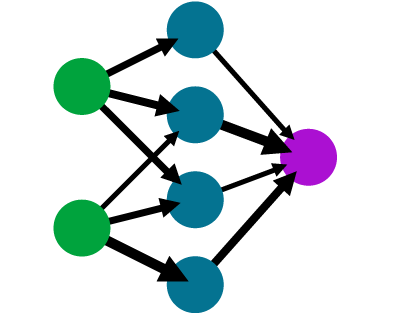
\includegraphics[width=3.125cm]{fig/photos/nn.png}};
\draw [ fill={rgb,255:red,218; green,221; blue,228}, fill opacity=1] (23.875,4.125) rectangle (25.375,3.375);
\node[anchor=center, align=center, fill={rgb,255:red,218; green,221; blue,228}, fill opacity=1, text opacity=1, inner xsep=0.080cm, inner ysep=0.085cm, rounded corners=0.020cm] at (24.625,3.75) {\fontsize{13.1pt}{17.0pt}\selectfont PID};
\draw [ fill={rgb,255:red,180; green,229; blue,254}, fill opacity=1, rounded corners = 12.6] (19.5,6.375) rectangle (22,4.875);
\node[anchor=center, align=center, inner xsep=0.095cm, inner ysep=0.085cm, rounded corners=0.020cm] at (20.75,5.625) {\fontsize{17.1pt}{22.2pt}\selectfont $\sqrt{T_i^{cmd}/k}$};
\draw [ color={rgb,255:red,255; green,0; blue,0}, draw opacity=1, line width=1.5pt, -{Stealth[scale=1.5]}, ] (7.375,15.5) -- (5.75,15.5);
\draw [line width=1.5pt, -{Stealth[scale=1.5]}, ] (5.75,16.375) -- (7.375,16.375);
\node [font=\fontsize{11.9pt}{15.5pt}\selectfont, fill={rgb,255:red,243; green,243; blue,243}, fill opacity=1, text opacity=1, inner xsep=0.080cm, inner ysep=0.085cm, rounded corners=0.020cm] at (9.125,15.5) {Backward Pass};
\node [font=\fontsize{11.9pt}{15.5pt}\selectfont, fill={rgb,255:red,243; green,243; blue,243}, fill opacity=1, text opacity=1, inner xsep=0.080cm, inner ysep=0.085cm, rounded corners=0.020cm] at (9,16.375) {Forward Pass};
\node [font=\fontsize{14.2pt}{18.5pt}\selectfont, fill={rgb,255:red,255; green,255; blue,255}, fill opacity=1, text opacity=1, inner xsep=0.080cm, inner ysep=0.085cm, rounded corners=0.020cm] at (22,16.1) {Translational};
\node [font=\fontsize{14.2pt}{18.5pt}\selectfont, fill={rgb,255:red,255; green,255; blue,255}, fill opacity=1, text opacity=1, inner xsep=0.080cm, inner ysep=0.085cm, rounded corners=0.020cm] at (21.75,19.525) {Rotational};
\node [font=\fontsize{18.2pt}{23.7pt}\selectfont, fill={rgb,255:red,255; green,255; blue,255}, fill opacity=1, text opacity=1, inner xsep=0.080cm, inner ysep=0.085cm, rounded corners=0.020cm] at (12,13.875) {$u_k$};
\node [font=\fontsize{18.2pt}{23.7pt}\selectfont, fill={rgb,255:red,243; green,243; blue,243}, fill opacity=1, text opacity=1, inner xsep=0.080cm, inner ysep=0.085cm, rounded corners=0.020cm] at (6.625,14.625) {$x_k$};
\node [font=\fontsize{11.9pt}{15.5pt}\selectfont, fill={rgb,255:red,243; green,243; blue,243}, fill opacity=1, text opacity=1, inner xsep=0.080cm, inner ysep=0.085cm, rounded corners=0.020cm] at (8.25,14.625) {State};
\node [font=\fontsize{11.9pt}{15.5pt}\selectfont, fill={rgb,255:red,243; green,243; blue,243}, fill opacity=1, text opacity=1, inner xsep=0.080cm, inner ysep=0.085cm, rounded corners=0.020cm] at (8.375,13.75) {Action};
\node [font=\fontsize{18.2pt}{23.7pt}\selectfont, fill={rgb,255:red,243; green,243; blue,243}, fill opacity=1, text opacity=1, inner xsep=0.080cm, inner ysep=0.085cm, rounded corners=0.020cm] at (6.625,13.75) {$u_k$};
\node [font=\fontsize{11.9pt}{15.5pt}\selectfont, fill={rgb,255:red,243; green,243; blue,243}, fill opacity=1, text opacity=1, inner xsep=0.080cm, inner ysep=0.085cm, rounded corners=0.020cm] at (9,12.75) {Loss Function};
\node [font=\fontsize{18.2pt}{23.7pt}\selectfont, fill={rgb,255:red,243; green,243; blue,243}, fill opacity=1, text opacity=1, inner xsep=0.080cm, inner ysep=0.085cm, rounded corners=0.020cm] at (6.625,12.75) {$\mathcal{L}()$};
\node [font=\fontsize{18.2pt}{23.7pt}\selectfont, fill={rgb,255:red,243; green,243; blue,243}, fill opacity=1, text opacity=1, inner xsep=0.080cm, inner ysep=0.085cm, rounded corners=0.020cm] at (6.625,11.75) {$\Gamma$};
\node [font=\fontsize{11.9pt}{15.5pt}\selectfont, fill={rgb,255:red,243; green,243; blue,243}, fill opacity=1, text opacity=1, inner xsep=0.080cm, inner ysep=0.085cm, rounded corners=0.020cm] at (9,11.75) {Allocation Matrix};
\end{circuitikz}